\chapter{Approach}\label{chapter:approach}

The goal of this work, was not only to replace \texttt{bicompose\_aux} by a safer version, but also to simplify it. While the general plan for the refactoring was fairly clear at the beginning, it seamed hard to figure out what features to cut, just based on looking at the code.

\section{Remove flatten}

To get a better understanding of how \texttt{bicompose\_aux} is used, we decided to add some statistics to \textit{Isabelle}. This way we found out how often each session called \texttt{bicompose\_aux} and what combination of flags each call had.

\begin{table}[ht]
\caption{Aggregated flag stats of Isabelle \texttt{3cc892b} and AFP \texttt{c0e959f}}
\begin{tabular}{*{5}{c} r}
flatten & match & incremented & lifted & eres\_flg & Quantity\\ \hline
False & True & False & False & False & 0.01\%\\
True & False & False & False & True & 0.03\%\\
False & False & False & False & False & 0.07\%\\
True & False & True & True & True & 1.43\%\\
True & False & False & False & False & 1.60\%\\
True & True & True & True & False & 1.83\%\\
True & True & True & True & True & 4.52\%\\
False & False & True & False & False & 9.51\%\\
True & False & True & False & False & 19.33\%\\
True & False & True & True & False & 61.66\%\\
\end{tabular}
\label{tab:agg_baseline}
\centering
\end{table}

Because we wanted to get a full picture, we built the whole \textit{Isabelle} distribution\footnote{\url{https://bitbucket.org/gnedl/isabelle-smashed}} and all of the sessions in the \textit{Archive of formal proof}\footnote{\url{https://bitbucket.org/gnedl/afp-smashed}}. For better comparability with later results, two session have been excluded, HOL-Proofs and HOL-Word-SMT\_Examples.\\
Even though the amount of different combinations might be overwhelming at first, things aren't as bad as they could be. Of the 25 possible configurations, only ten are used in practice. To make matters even easier, the top three combinations are used in 90\% of all cases. While It may also seam apparent, that many of the more obscure configurations effectively not used, it should not be forgotten, that at 8077146288 invocations, one basis point still accounts for a meaningful amount of calls to \texttt{bicompose\_aux}.

\begin{table}[ht]
\caption{Frequency of flags set over all invocations in Isabelle \texttt{3cc892b} and AFP \texttt{c0e959f}}
\begin{tabular}{l r}
flatten & 90.4\%\\
match & 6.4\%\\
incremented & 98.3\%\\
lifted & 69.4\%\\
eres\_flg & 6.0\%
\end{tabular}
\label{tab:flag_freq}
\centering
\end{table}

When aggregating by the flags, it can be observed, that all but the lifted flag have a clear tendency with regard to being true or false in general. These should be easier to remove, because even a costly alternative might not be prohibitively expensive.\\
While match would fit that bill, instead of doing this check on the unifier, it could be performed on the resulting theorem, it is not practical. Because a new version of \texttt{bicompose\_aux} would not require this to be a feature within the kernel, pulling it further out, would only decrease the versatility of the new \texttt{bicompose\_aux}, while impeding performance with the costlier check.\\
Incremented does not influence trusted code, but for the optimization to have actual benefits, needs to be know when the unifiers are generated, this is only possible within \texttt{bicompose\_aux}. Because it is not possible to increment all theorem for compatibility reasons, it would have to be disable. This would decrease speed in 98.3\% of all invocations.\\
When performing beta normalization at the end, lifting needs to be considered to stay compatible. Thus the lifting flag needs to retain its current form.\\
It is conceivable to do elim-resolution outside of \texttt{bicompose\_aux} but there is some performance to be lost, because the elim part is conceptually part of the resolution. While the two could be separated, the resulting code duplication is undesirable.\\
Flatten is the one interesting case, because there is only a handful of points in the code base, where it is not enabled. Tree have to do with adding or removing protect markers and the one outlier is \texttt{distinct\_tac}. It seams to be used for deleting duplicate subgoals, but evidently doesn't depend on getting unflattend theorems. No functionality depending on it seams to suffer from the change either.\\
All functions dealing with protection markers in any way, use the definition of the marker $\#(\text{PROP}~?A) \equiv \text{PROP}~?A$ to resolve with. As the definition is only used on premises, the conclusion or tailing premises and the conclusion, this can be simulated using existing primitives. By using to \texttt{combination} rule to skip the static premises, and using \texttt{instantiate} on the definition with the protectee as the substitution. An example for such a proof is removing a marker as done by Goal.conclude, which can be found in figure~\ref{fig:conclude}. The size of the proof depends on the number of skipped subgoals and is hidden by the derived rule combination*.

\begin{figure}[ht]
% \begin{displaymath}
% \scalebox{.8}{
%     \prfinterspace = 1em
%     \prftree[r]{$\equiv$-elim}
%     {
%         \prftree[r]{$\beta$-norm}
%         {
%             \prftree[summary]
%             {\texttt{GOAL}}
%         }
%         {\texttt{GOAL} \equiv \beta\left(\texttt{GOAL}\right)}
%     }
%     {
%         \prftree[r]{$\equiv$-elim}
%         {
%             \prftree[r]{combination*}
%             {
%                 \prftree[r]{reflexivity}
%                 {\texttt{PRE} \equiv \texttt{PRE}}
%             }
%             {
%                 \prftree[r]{instantiation}
%                 {\prfbyaxiom{prop\_def}{\#(\text{PROP}~?A) \equiv \text{PROP}~?A}}
%                 {\#\left(\texttt{SAFE}\right) \equiv \texttt{SAFE}}
%             }
%             {\texttt{IN} \equiv \texttt{GOAL}}
%         }
%         {\texttt{IN}}
%         {\texttt{GOAL}}
%     }
%     {\beta\left(\texttt{GOAL}\right)}
% }
% \end{displaymath}
\centering
\newcommand\GOAL{\mathit{GOAL}}
\newcommand\PRE{\mathit{PRE}}
\newcommand\SAFE{\mathit{SAFE}}
\newcommand\IN{\mathit{IN}}
\scalebox{.73}{
\begin{prooftree}
%   \Infer0[reflexivity]{\texttt{PRE} \equiv \texttt{PRE}}
%   \Infer0[prop\_def]{\#(\text{PROP}~?A) \equiv \text{PROP}~?A}
%   \Infer1[instantiation]{\#\left(\texttt{SAFE}\right) \equiv \texttt{SAFE}}
%   \Infer2[combination*]{\texttt{IN} \equiv \texttt{GOAL}}
  % \Hypo{$\vdots$}
  % \Infer1[$\equiv$-elim]{\GOAL}
  \Infer0[$\beta$-norm]{\GOAL \equiv \beta\left(\GOAL\right)}

  \Infer0[reflexively]{\PRE \equiv \PRE}
  \Infer0[prop\_def]{\#(\text{PROP}~?A) \equiv \text{PROP}~?A}
  \Infer1[instantiation]{\#\left(\SAFE\right) \equiv \SAFE}
  \Infer2[combination*]{\IN \equiv \GOAL}
  \Hypo{\IN}
  \Infer2[$\equiv$-elim]{\GOAL}
  \Infer2[$\equiv$-elim]{\beta\left(\GOAL\right)}
\end{prooftree}
}
\begin{align*}
  \text{where}~\GOAL &::= \left\llbracket A_x\,\middle|\, x \in \left[ m \right] \right\rrbracket \Longrightarrow C \\
  \PRE &::= \left\llbracket A_x\,\middle|\, x \in \left[ i \right] \right\rrbracket \Longrightarrow \\
  \SAFE &::= \left\llbracket A_x\,\middle|\, x \in \left( \left[ m \right] \setminus \left[ i \right] \right)\right\rrbracket \Longrightarrow C \\
  \IN &::= \PRE~\left(\#\SAFE\right)
\end{align*}
\caption{Goal.conclude}
\label{fig:conclude}
\end{figure}

% \begin{displaymath}
% \scalebox{.2}{
%     \prftree%[r]{$\equiv$-elim}
%     {\left\llbracket A_x\,\middle|\, x \in \left[ m \right] \right\rrbracket \Longrightarrow B}
%     {
%         \prftree%[r]{$\equiv$-elim}
%         {
%             \prftree%[r]{combination*}
%             {
%                 \prftree%[r]{reflexivity}
%                 {
%                     \left\llbracket A_x\,\middle|\, x \in \left[ i \right] \right\rrbracket \Longrightarrow
%                         \equiv \left\llbracket A_x\,\middle|\, x \in \left[ i \right] \right\rrbracket \Longrightarrow}
%                 \prftree%[r]{instantiation}
%                 {
%                     \#\left( \left\llbracket A_x\,\middle|\, x \in \left( \left[ n \right] \setminus \left[ i \right] \right)\right\rrbracket \Longrightarrow C \right)
%                     \equiv \left\llbracket A_x\,\middle|\, x \in \left( \left[ n \right] \setminus \left[ i \right] \right)\right\rrbracket \Longrightarrow C
%                 }
%             }
%             {\left\llbracket A_x\,\middle|\, x \in \left[ i \right] \right\rrbracket \Longrightarrow \#\left( \left\llbracket A_x\,\middle|\, x \in \left( \left[ n \right] \setminus \left[ i \right] \right)\right\rrbracket \Longrightarrow C \right)
%             \equiv \left\llbracket A_x\,\middle|\, x \in \left[ m \right] \right\rrbracket \Longrightarrow C}
%         }
%         {\left\llbracket A_x\,\middle|\, x \in \left[ i \right] \right\rrbracket \Longrightarrow \#\left( \left\llbracket A_x\,\middle|\, x \in \left( \left[ n \right] \setminus \left[ i \right] \right)\right\rrbracket \Longrightarrow C \right)}
%         {\left\llbracket A_x\,\middle|\, x \in \left[ m \right] \right\rrbracket \Longrightarrow C}
%     }
%     {\beta\left( \left\llbracket A_x\,\middle|\, x \in \left[ m \right] \right\rrbracket \Longrightarrow C \right)}
% }
% \end{displaymath}

\section{New bicompose\_aux}

By dividing \texttt{bicompose\_aux} into the sub tasks found in \ref{fig:flow}, the process as a whole should be more accessible. For each of those tasks, many different approaches are feasible and some of those will be discussed in the following.

\begin{figure}[ht]
\centering
\usetikzlibrary{arrows, decorations.markings}
\tikzstyle{vecArrow} = [thick, decoration={markings,mark=at position
   1 with {\arrow[semithick]{open triangle 60}}},
   double distance=1.4pt, shorten >= 5.5pt,
   preaction = {decorate},
   postaction = {draw,line width=1.4pt, white,shorten >= 4.5pt}]
\tikzstyle{innerWhite} = [semithick, white,line width=1.4pt, shorten >= 4.5pt]
\usetikzlibrary{positioning}
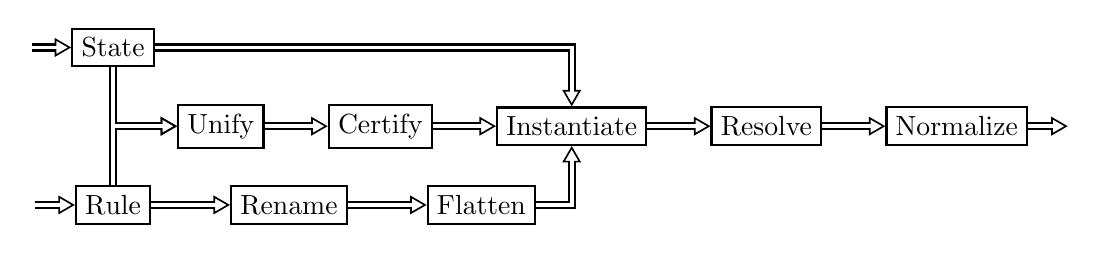
\begin{tikzpicture}[thick]
  \node[draw,rectangle] (rule) {Rule};
  \node[inner sep=0,minimum size=0,left=0.5cm of rule] (pr) {}; % invisible node
  \node[inner sep=0,minimum size=0,above of=rule] (k) {}; % invisible node
  \node[draw,rectangle,above of=k] (state) {State};
  \node[inner sep=0,minimum size=0,left=0.5cm of state] (ps) {}; % invisible node
  \node[draw,rectangle,right=of rule] (rename) {Rename};
  \node[draw,rectangle,right=0.8cm of k] (unify) {Unify};
  \node[draw,rectangle,right=of rename] (flatten) {Flatten};
  \node[draw,rectangle,right=0.8cm of unify] (certify) {Certify};
  \node[draw,rectangle,right=0.8cm of certify] (inst) {Instantiate};
  \node[draw,rectangle,right=0.8cm of inst] (res) {Resolve};
  \node[draw,rectangle,right=0.8cm of res] (norm) {Normalize};
  \node[inner sep=0,minimum size=0,right=0.5cm of norm] (pn) {}; % invisible node

  % 1st pass: draw arrows
  \draw[vecArrow] (pr) to (rule);
  \draw[vecArrow] (ps) to (state);
  \draw[vecArrow] (state) |- (unify);
  \draw[vecArrow] (rule) |- (unify);
  \draw[vecArrow] (rule) to (rename);
  \draw[vecArrow] (rename) to (flatten);
  \draw[vecArrow] (state) -| (inst);
  \draw[vecArrow] (flatten) -| (inst);
  \draw[vecArrow] (unify) to (certify);
  \draw[vecArrow] (certify) to (inst);
  \draw[vecArrow] (inst) to (res);
  \draw[vecArrow] (res) to (norm);
  \draw[vecArrow] (norm) to (pn);

  % 2nd pass: copy all from 1st pass, and replace vecArrow with innerWhite
  \draw[innerWhite] (state) to (rule);

  % Note: If you have no branches, the 2nd pass is not needed
\end{tikzpicture}
\caption{Information Flow}
\label{fig:flow}
\end{figure}

\subsection{Equality}

Before any other word can be lost on resolution, the crucial equality check that underlies any sensible concept need to be discussed. A general equality test for the propositions, or sub propositions, of two given theorems has to overcome many hurdles. Starting with syntactic equivalence of lambda representation of the \textit{Pure} terms, the notion of equivalence needs to be broadened. Most of these are well known and will only be mentioned briefly.\\
$\equiv_\alpha$ ignores the name of bound variables. This is particularly easy in this case, because the terms use De Bruijn indices. With these indices bound locally bound variables don't have the name of their binder associated, but the distance to their binder. In general the binders wouldn't need to have a string associated to them, but for improved readability of the terms, they have all have a name. All that needs to be done for $\equiv_\alpha$ is to descend both terms in parallel and ignore the labels of the binders.\\
During $\beta$ normalization possible function applications are performed. This means, that the term is rewritten, using $(\lambda a.u) t \rightarrow u[t \backslash a]$. After $\beta$ normalizing two terms, they can be checked for $\equiv_\beta$, by the simple equivalence test. The approach to establish $\equiv_\eta$ is practically the same. Here a different kind of unnecessary abstractions are removed by applying $(\lambda a.f a) \rightarrow f$.\\
To yield $\equiv_{\alpha\beta\eta}$ the arguments are both $\beta$ and $\eta$ reduced and then checked for $\equiv_\alpha$. While all these are necessary to check equivalence of terms that are considered equal, they are not sufficient. This is due to a specialty of the higher-order unification in \textit{Isabelle}. In some cases, when there is not one clear way to solve an equation, the unifier will, along with the actual substitutions, return a list of flex-flex pairs. These are pairs of possible sub terms that should be assumed to allow for a unifier. A finished lemma will generally not contain any, as the veracity of its proposition is dependant on the flex-flex pairs being solvable. Thus placing even more trust in the unifier.\\
While coming up with an algorithm to test for equality modulo flex-flex pairs will eventually be needed, it turns out that in almost all cases these equations can be smashed immediately~\parencite{Wimmer2016}. Smashing extents the unifier in one possible way to solve the pair and thus makes dealing with these pairs in \texttt{bicompose\_aux} unnecessary.

\subsection{Resolution}

The idea of this function is to use the modus ponens rule backwards on subgoal $i$ of the state. Any reasonable way to implement this, must include a equality check, which will be discussed in the next subsection.

\subsubsection{Old primitives}

While we were able to come up with proofs using existing primitives exclusively, they all depend on the use of the $\Longrightarrow$-intro rule. The thing problematic about this, is that it pulls the term that is added to the premises of the proposition out of the hypothesis of the theorem. This is only a problem, because terms in the hypothesis can't contain schematic variables. While this could theoretically be circumvented by temporarily converting the schematic variables to free ones, it's not a clean solution.

\subsubsection{New primitive with $\equiv_\alpha$}

By introducing a new primitive that performs this generalized modus ponens directly on two theorems, some performance gains can be expected. Because $B$ and $B_i$ are required to be equal, it needs to be checked when using this primitive. Other \textit{Pure} primitives that require such a check, like $\equiv$-elim and $\Longrightarrow$-elim, use \texttt{aconv} for this. It tests two terms for $\equiv_\alpha$. For uniformity and because it's already part of the kernel, it would be the canonical choice. The drawback is, that it will only admit a proper subset of the possible inputs expected to work.\\
To get around that, either $B$ must be safely exchanged with $B_i$ in the rule, or vice versa. To do this the existing primitives \texttt{beta\_conversion} and \texttt{eta\_conversion} can be used, or a new one, that does both can be created.

\begin{figure}[ht]
\newcommand\A{\left\llbracket A_x\,\middle|\, x \in \left[ m \right] \right\rrbracket \Longrightarrow}
\centering
\scalebox{0.86}{
\begin{prooftree}
%   \Infer0[reflexivity]{\texttt{PRE} \equiv \texttt{PRE}}
%   \Infer0[prop\_def]{\#(\text{PROP}~?A) \equiv \text{PROP}~?A}
%   \Infer1[instantiation]{\#\left(\texttt{SAFE}\right) \equiv \texttt{SAFE}}
%   \Infer2[combination*]{\texttt{IN} \equiv \texttt{GOAL}}

      \Infer0[reflexively]{A \equiv A}

        % \Hypo{B}
        \Infer0[$\beta\eta$-norm]{B \equiv \eta\left(\beta\left(B\right)\right)}

        % \Hypo{B_i}
        \Infer0[$\beta\eta$-norm]{B_i \equiv \eta\left(\beta\left(B_i\right)\right)}
        \Infer1[symmetry]{\eta\left(\beta\left(B_i\right)\right) \equiv B_i}

      \Infer2[transitivity]{B \equiv B_i}

    \Infer2[combination*]{A B \equiv A B_i}

    \Hypo{A B}
  
  \Infer2[$\equiv$-elim]{A B_i}
\end{prooftree}
}
\begin{align*}
  \text{where}~A &::= \left\llbracket A_x\,\middle|\, x \in \left[ m \right] \right\rrbracket \Longrightarrow
\end{align*}
\caption{Replace $B$ by $B_i$ in the rule}
\label{fig:replace_b}
\end{figure}


\subsubsection{New primitive with $\equiv_{\alpha\beta\eta}$}

To make this procedure even faster, the primitive could perform the stronger equality check itself. Not only would the substitution, necessary when dealing with the previous version, be obsolete, the equality check itself can also be improved upon. By performing the more expensive $\beta$/$\eta$-conversions only if the previous failed, some savings can be achieved.

\subsection{Certify}

To prepare an environment returned by the unification algorithm, some steps need to be taken.\\
The first issue is, that the substitution in the environment is in triangular form. Under this circumstance, it isn't guaranteed, that the sets of variables on the left and the right of the substitution are disjoint. When this is the case, instantiating a term with such a substitution again might generate a different result. An obviously correct solution to this is to instantiate until a fixpoint is found. But as accessible it might be, there is a more efficient version. The idea is to substitute the variables in the intersection of the two sets with their respective definitions on the right sides of the substitutions. This act is often referred to as chasing. Once the type and term substitutions have been chased, they can be certified using \texttt{global\_ctyp\_of} and \texttt{global\_cterm\_of}.

\subsection{Additional Primitives}

For the remaining tasks the correct approach is clear, either because they exist already or don't have the appropriate generality.

\subsubsection{Rename} There are primitives for both renaming bound and schematic variables. \texttt{renamed\_prop} allows the user to exchange the proposition of a theorem with one that is $\equiv_\alpha$ and instantiate can be used to rename schematic variables. This means current logic needs to be separated by variable kind. The part that deals with bound variables can remain unchanged and it's result can be used as input for \texttt{renamed\_prop}. For the other kind, the substitutions need to be generated from the existing lists.
\subsubsection{Flatten} Flattening is not used outside of \texttt{bicompose\_aux} and there seams to be little need for it. Therefore are primitive that performs flattening exactly as needed by \texttt{bicompose\_aux} is reasonable.
\subsubsection{Unify} Prepares the environment for the unification algorithm and retrieves the unifier. There is not trusted code here, as the unifier is later checked.
\subsubsection{Instantiate} Is just a call to the existing primitive.
\subsubsection{Normalize} The existing \texttt{beta\_conversion} can be used for reducing the complete proposition of a theorem, but previous optimizations require more control over the affected subgoals. This can be accommodated by proof similar to ones in the goal protection family.